\documentclass[10pt,a4paper]{article}
\usepackage[margin=2cm]{geometry}
\usepackage{graphicx,booktabs,amsmath,hyperref,float}
\title{Learned Page Replacement When the Workload Changes}
\author{Oyon \quad (ID: 202414054)\\ Dept. of CSE, MIST\\ CSE-307 Term Paper, Track 1}
\date{4 October 2026}
\begin{document}
\maketitle
\begin{abstract}
In this term paper I implement FIFO, LRU and Optimal page replacement and add a small decision-tree policy that learns which page to evict. I test them on a trace where the access pattern changes in the middle, from locality-heavy to random. The learned policy is about as good as LRU before the change and a bit worse after it.
\end{abstract}

\section{Introduction}
When memory is full and a page fault happens, the OS has to remove one page to make room. FIFO removes the page that was loaded first, LRU removes the page not used for the longest time, and Optimal (Belady's algorithm) removes the page whose next use is farthest away \cite{belady1966,silberschatz}. Optimal cannot be used in a real system because it needs the future, but it shows the best possible result. Some recent work tries to improve caching with machine learning predictions \cite{lykouris2018}. In this paper I check what happens to these policies when the workload changes after some time.

\section{Implementation}
The code is written in Python. FIFO uses a queue, LRU uses an ordered dictionary, and Optimal first computes the next use of every reference and then evicts the page with the largest value. I checked all three on the example reference string from the textbook with 3 frames and got 15, 12 and 9 faults for FIFO, LRU and Optimal \cite{silberschatz}.

For the learned policy, every page in memory has four features at the time of a fault: how long ago it was last used, how many times it was used in the last 100 references, how long it has been in memory, and how many times it was used since it was loaded. A decision tree of depth 4 from scikit-learn \cite{pedregosa2011} predicts if the page will not be used again in the next 40 references. The training labels are found by looking at the future of a training trace. When a fault happens, the page with the highest chance of not being used soon is evicted. I made two versions:
\begin{itemize}
\item Learned-static: trained once on a separate trace that has only the first pattern.
\item Learned-online: retrained every 1000 references using only the last 3000 references.
\end{itemize}

\section{Experiment}
Each trace has 20000 references over 200 pages and the memory has 20 frames. In the first half, most references (90\%) go to a small working set of 12 pages that moves slowly, and the rest are a sequential scan. In the second half, pages are chosen uniformly at random, and sometimes a short burst of 5 to 20 references goes to a group of 3 pages. I ran 20 different random seeds and report the average hit ratio and number of page faults for each half.

\section{Results}
\begin{table}[H]\centering
\caption{Mean hit ratio and page faults over 20 seeds (each phase has 10{,}000 references).}
\begin{tabular}{lcccccc}\toprule
Policy & Hit (before) & Hit (after) & Rel.\ drop & Faults (before) & Faults (after) & Faults (total)\\\midrule
FIFO & 0.814 & 0.371 & 54.4\% & 1863 & 6288 & 8151\\
LRU & 0.883 & 0.372 & 57.9\% & 1167 & 6285 & 7452\\
Learned-static & 0.889 & 0.341 & 61.7\% & 1115 & 6593 & 7708\\
Learned-online & 0.888 & 0.355 & 60.1\% & 1119 & 6452 & 7571\\
OPT & 0.905 & 0.561 & 38.0\% & 955 & 4389 & 5344\\\bottomrule
\end{tabular}\end{table}

\begin{figure}[H]\centering
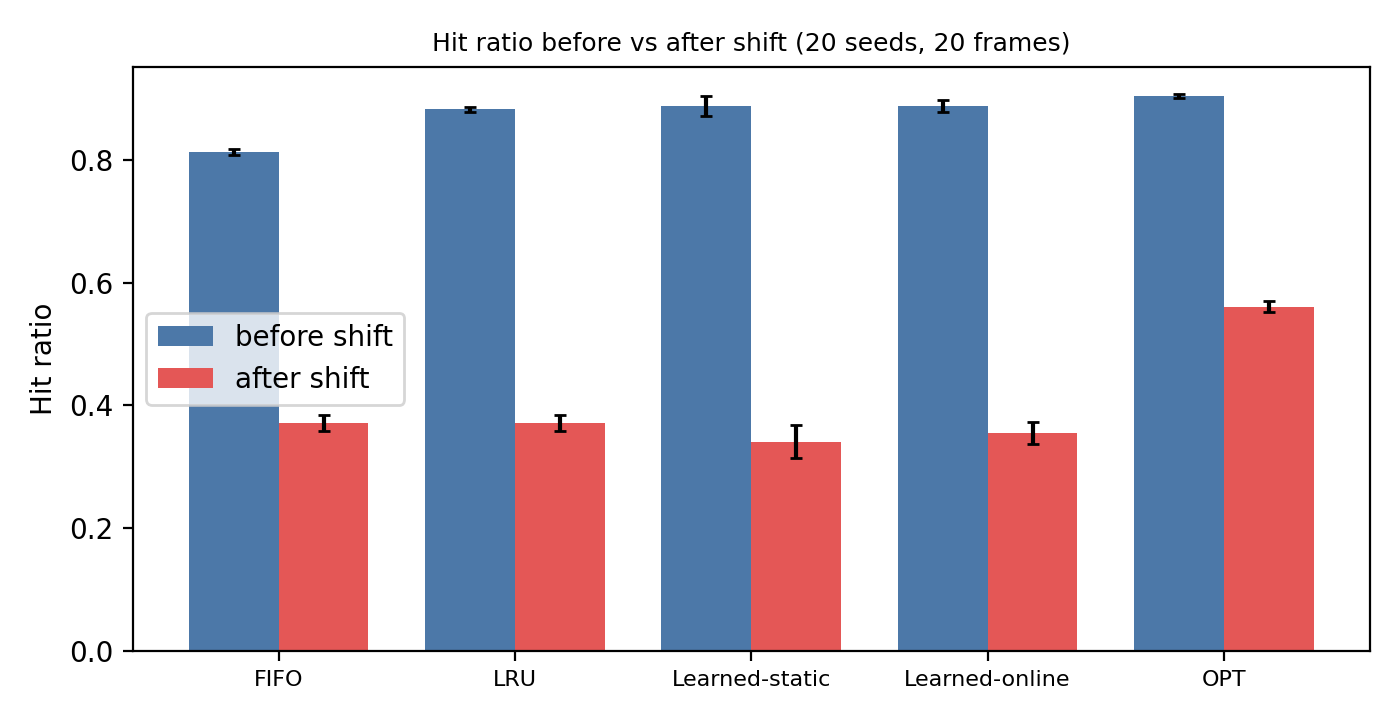
\includegraphics[width=0.78\linewidth]{fig_hit_ratio_phases.png}
\caption{Hit ratio before and after the shift (error bars: std over seeds).}\end{figure}
\begin{figure}[H]\centering
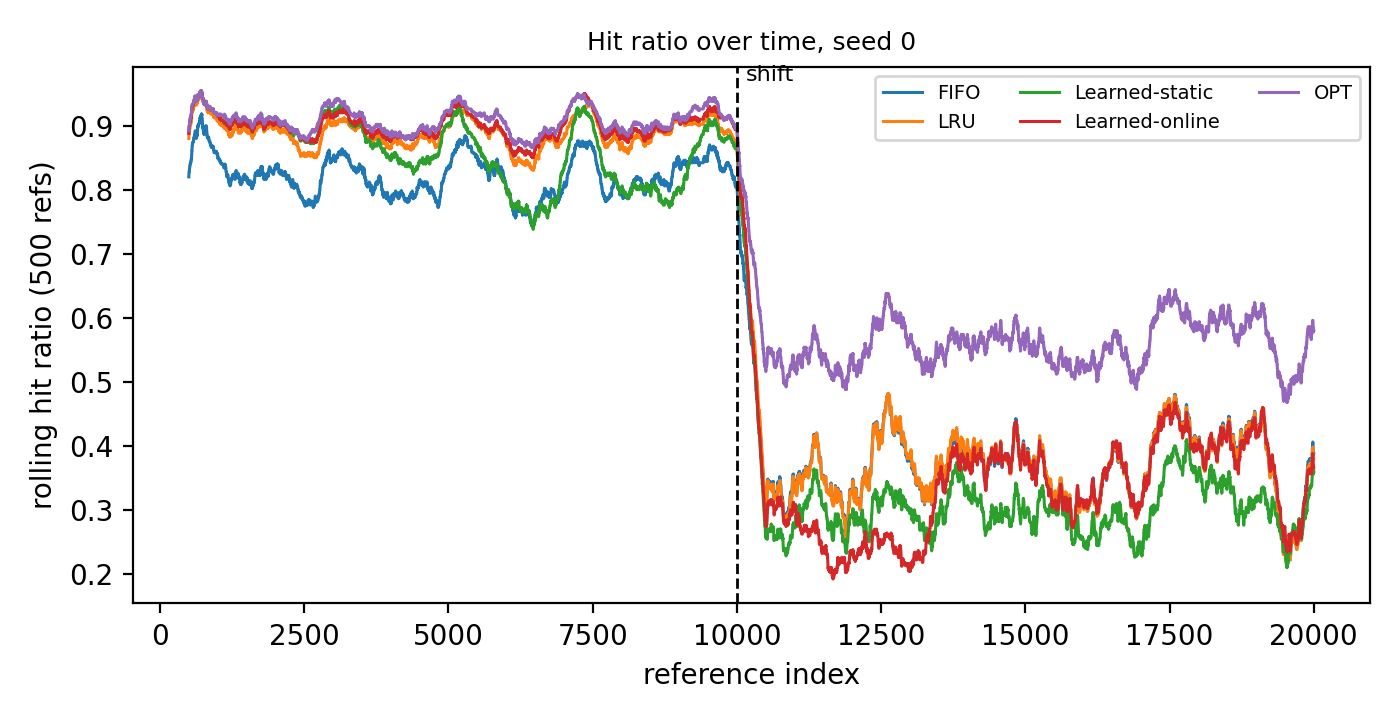
\includegraphics[width=0.78\linewidth]{fig_rolling_hit_ratio.png}
\caption{Rolling hit ratio (window 500) for one seed; dashed line marks the shift.}\end{figure}

\section{Analysis}
Before the shift, LRU (0.883) is clearly better than FIFO (0.814). The reason is that FIFO can remove a page of the working set just because it was loaded long ago, even if it is used all the time. The learned policy (0.889) is about the same as LRU and close to Optimal (0.905).

After the shift, every policy gets much worse. Pages are now chosen randomly from 200 pages while only 20 fit in memory, so there is no page that is more likely to come back than another, and the recent history does not help. Because of this FIFO and LRU give almost the same result (0.371 and 0.372). Optimal still reaches 0.561 because it knows the future, including the bursts.

In relative terms the learned static policy dropped the most (61.7\%), then the online one (60.1\%), then LRU (57.9\%) and FIFO (54.4\%). FIFO has a smaller drop only because it started lower. Optimal dropped the least (38.0\%). I think the learned policy suffers more because it learned rules from the first pattern, like keeping pages that are used often, and these rules do not work when the pages are random. Retraining online helped a little (0.355 against 0.341), but it was still below LRU, probably because the recent data contains the change itself and the random part has little to learn from.

The experiment has some limits: the traces are synthetic, there is only one shift and one memory size, and I used only one type of model. Also the learned policy did not give a big gain even before the shift, so for this kind of workload LRU is already quite good.

\begin{thebibliography}{9}
\bibitem{belady1966} L.~A. Belady, ``A study of replacement algorithms for a virtual-storage computer,'' \emph{IBM Systems Journal}, 5(2):78--101, 1966.
\bibitem{silberschatz} A.~Silberschatz, P.~B. Galvin, G.~Gagne, \emph{Operating System Concepts}, 10th ed., Wiley, 2018.
\bibitem{lykouris2018} T.~Lykouris and S.~Vassilvitskii, ``Competitive caching with machine learned advice,'' in \emph{ICML}, 2018.
\bibitem{pedregosa2011} F.~Pedregosa et al., ``Scikit-learn: Machine learning in Python,'' \emph{JMLR}, 12:2825--2830, 2011.
\end{thebibliography}
\end{document}
